\documentclass[11pt,oneside,a4paper,notitlepage]{article}

\usepackage[utf8]{inputenc}
\usepackage[ngerman]{babel}
\usepackage[margin=1.5cm]{geometry}

%kommentare, zitate, quellcode
\usepackage{verbatim}
%\fontfamily{sfdefault}
\renewcommand{\familydefault}{\sfdefault}
%
\usepackage{graphicx}
%fuer tabellen
\usepackage{tabularx}
\usepackage{tabulary}
%
%formatierung listen
\let\oldenumerate\enumerate
\renewcommand{\enumerate}{
  \oldenumerate
  \setlength{\itemsep}{1pt}
  \setlength{\parskip}{0pt}
  \setlength{\parsep}{0pt}
}

%
%referenzen und links
\usepackage{hyperref}
\hypersetup{
colorlinks=false,
hidelinks=false
}
%
% 
\renewcommand{\arraystretch}{1.5}
%

\begin{document}


\section{Deskriptives Kommunikationsmodell}

Das Modell beschreibt die Kommunikationsvorgänge zwischen den identifizierten Stakeholdern im Rahmen der Prozesse die aus der Recherche zur Anwendungsdomäne, der Marktanalyse und den Gesprächsprotokollen entnommen wurden.


\subsection*{Scanner}
Scannen Dokumente ein und leiten diesen einen OCR-Erkennungsprozess weiter.

\subsection*{Erfasser}
Erhalten Dokumente aus dem Erkennungsprozess und korrigieren diese oder führen eine vollständige Erfassung eines
Dokumentes durch und leiten dieses an die Verwaltungsangestellten weiter.


\subsection*{Verwaltungsangestellte}
Erhalten Dokumente von den Erfassern und nutzen ein betriebliches Anwendungssystem um diese mit Attributen zu versehen und 
einem Geschäftsvorgang zuzuordnen. Geben den Geschäftsvorgang an einen Fachangestellten weiter. Stellen bei Problemen mit der Zuweisung oder Attributtierung Rückfragen an Fachangestellte oder in kritischen Fällen an einen Entscheider.


\subsection*{Fachangestellte}
Erhalten einen Geschäftsvorgang von Verwaltungsangestellten oder Fachangestellten und ordnen diesem Vorgangs- oder Fachbezogene Attribute zu. Beantworten Rückfragen der Fachangestellten und wenden sich bei Problemen mit der Zuweisung an einen entsprechenden Entscheider.


\subsection*{Entscheider}
Erhalten durch Berichte und Besprechungen Einsicht in bestehende Prozesse und greifen per Anweisung an Verwaltungs- und Fachangestellte in einen Prozess ein. Teilen den Angestellten bei Vorgangsproblemen die durchzuführende Lösung des Problems mit.

\section{Kommunikationsdiagramm}

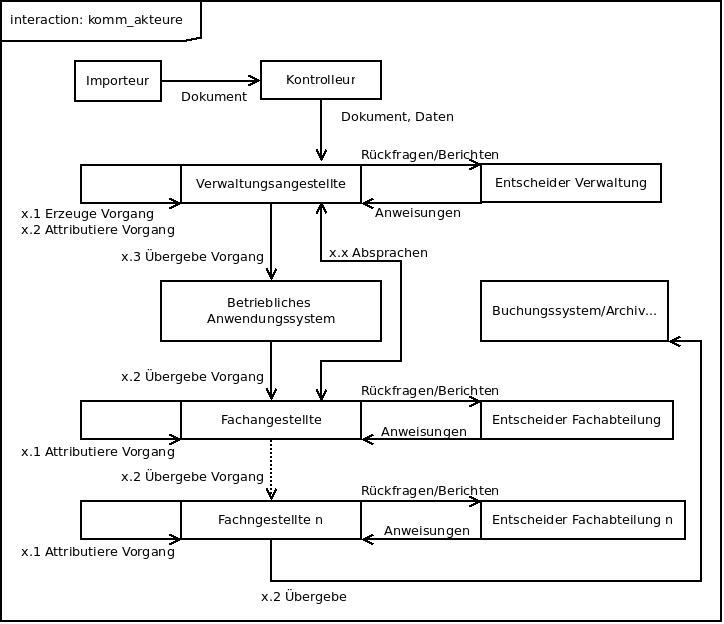
\includegraphics[width=\textwidth]{EISWS1516Howe_Kommunikation_deskriptiv.png}
\noindent

\end{document}

